
\documentclass[11pt]{article}
\usepackage{amsmath,textcomp,amssymb,geometry,graphicx}

\def\Name{Stefan Isenberger}  % Your name
\def\Login{ee122-dx} % Your login

\title{EE122--Fall 2013 --- Solutions to Homework 1}
\author{\Name, \texttt{\Login}}
\markboth{EE122--Fall 2013 Homework 1 \Name}{EE122--Spring 2013 Homework 1 \Name, \texttt{\Login}}
\pagestyle{myheadings}

\begin{document}
\maketitle

\section*{1.}

\begin{itemize}
\item[(1)] \textbf{22.4 milliseconds.}

Bits must travel $6*10^5$ meters at a speed of $3*10^8$ $\frac{m}{s}$, which gives a propagation delay of 20ms. Packets of size 1200 bytes (or 9600 bits) over a $4*10^6$ bit channel will incur a transmission delay of 2.4 milliseconds. Thus, the total delay to send a packet from A to B will be 22.4 milliseconds.
\item[(2a)] \textbf{21.22 seconds}

A 10MB file being sent as 1060 byte packets will be transmitted completely after 10000 packets. The propagation delay is the same for this link as it was in the previous question, but the transmission delay will change (because packets are now 1060 bytes). The transmission delay for the new packets will be 2.12 ms (which is $\frac{1060*8}{4*10^6}$ seconds). Adding up all of these transmission delays for each packet gives a total delay for the message of $.00212*10000=21.2$ seconds. Finally, the last packet will arrive at B after its propagation delay has elapsed, 20 ms later. The total time for the file transmission is thus 21.22 seconds.
\item[(2b)] \textbf{The "goodput" is 3.77 Mbps}

Since it takes 21.22 total seconds to send a file of size $8*10^7$ bits, the useful bits will arrive at a rate of $\frac{8*10^7}{21.22}=3.77$ Mbps. 
\item[(3)] \textbf{42.41 milliseconds}

The transmission delay for the 1000 byte packet is $\frac{8000}{4*10^6}=2$ms. It will then take a propagation delay of 20 ms to reach B. B will then process the packet for .25ms. B's acknowledgement packet will have its own transmission delay of .16 ms, and will finally reach A after the propagation delay of 20ms. The sum of all these delays is 42.41 ms from when A began sending its original packet.
\item[(4)] \textbf{421.6 milliseconds}

A will send 10 packets. Transmitting each packet takes enough time for both the packet travelling from A to B and the acknowledgement from B to A. As we saw in the question before, since both routes have the same propagation delay, the total time to send a 1000 byte packet and receive acknowledgement is 2+20+.16+20=42.16 milliseconds. Since 10 of these packets must be sent and acknowledged, the total time to send and acknowledge the entire file will be 421.6 ms.
\end{itemize}

\section*{2.}

\begin{itemize}
\item[(1)] \textbf{108 milliseconds}

The transmission delay of a 1500 byte (or 12000 bit) packet from Alice to A is 12 ms, from A to B is 24 ms, from B to C is 12 ms, and from C to Bob is 6 ms. The sum of all latencies is 2 + 20 + 30 + 2 = 54 ms. Thus, the total transmission of a single 1500 byte packet on an empty network from Alice to Bob is 54 + 12 +24 +12 + 6 = 108ms.
\item[(2)] \textbf{156 milliseconds}

The transmission delay on the link from Alice to A is 12 ms. However, from A to B, it is 24 ms. Thus, the second packet reaching B must be queued up before it is sent out, since the first packet will not have sent yet. The second packet will arrive at A at 24+2=26 ms from the starting point. However, the first packet will not finish leaving A until 14+24=38ms. Thus, there is a 12ms queueing delay on the second packet, before it finally leaves A at 38+24=62ms. By this time, the third packet will be queued up, and it will itself leave A 24ms later, at 86ms. Since all the rest of the links have higher capacity outgoing than incoming, there will be no more queueing delays, and the final packet will simply have to deal with a 20 ms latency from A to B, a 12 ms transmission delay from B to C, a 30ms latency from B to C, a 6 ms trans. delay from C to Bob, and a 2ms latency from C to Bob, arriving at 86+20+12+30+6+2=156ms from the start point.
\item[(3a)] \textbf{14 arrive, 6 are dropped}

Packets arrive twice as fast as they are sent out at the link at A. What this means is that when one packet has been entirely sent out, two new packets have arrived. Thus, every 24ms (the transmission delay out of A), the number of packets in the queue has increased by 1. After the first 24 ms, there will be one packet in the queue, and one beginning its transmission. This means that after 24*4=96ms, there will be 4 packets in the queue, and one beginning its transmission. 12ms later, another packet will reach the queue. However, the transmitting packet will not have left yet, so the queue will be full, and the next incoming packet will be dropped. This first dropped packet is packet nine. After this, the queue will have an open spot on only half of the incoming packets. Since there are 11 packets left, this corresponds to 5 more dropped packets, for 6 total dropped. 
\item[(3b)] \textbf{Packets 9, 11, 13, 15, 17, and 19 are dropped} (assuming that packets can be moved instantaneously from the queue to the transmission, and that such a delay doesn't cause packets to be in the queue and hog spots when there's technically openings).
\item[(4)] \textbf{25\% of Bob's packets make it to Alice}

From Bob's end, there will be queueing delays at both C and B, since the incoming link (from his side) is faster than the outgoing. As we saw with Alice, after an initial amount of setup packets to fill the queue, packet dropping behavior happens at a simple ratio. In this case, like Alice's, the outgoing connection from C transmits packets at half the rate as they come in. This means, ones the queue is full, that the queue will be full for 1 out of every two incoming packets to C. Thus, in the case of an infinite stream of packets, well after the queue-filling time, $50\%$ of packets at C will be dropped.

However, the link at B also transmits at $50\%$ of the rate as its incoming packets from C. This means that, once B's queue has reached a steady state, it will also drop $50\%$ of its incoming packets. 

Once a packet is through B, it is guaranteed to reach Alice (at least without faulty wiring) because the link to Alice from A is faster than the incoming link from B.

Thus, one half of Bob's packets make it through C, of which another $50\%$ will be dropped at B (as the number of sent packets goes to infinity). Bob's successful packet transfer is $25\%$.
\item[(5a)]\textbf{228 milliseconds}

Alice's worst case queuing delay is the case in which a packet fills the queue at A at exactly the same time that a packet begins transmitting out of A. In this case, the packet will have to wait for five packets to transmit (a 5*24=120ms) queueing delay before it can transmit. However, since no other switches have queueing delays, the end to end latency for a packet in the worst case is simply the end-to-end on an empty network plus a 120ms queueing delay, which is 108+120=228ms
\item[(5b)] \textbf{288 milliseconds}

In Bob's worst case end-to-end latency, packets will be stuck in the queue at both C and B and have to wait for a full queueing delay at both. The queuing delay at C will be 5 times the transmission delay of 12ms, or 60ms. The worst-case queueing delay at B will be 5*24ms, for 120ms. Thus, the worst case packet end-to-end latency for a packet sent from Bob to Alice is 108ms + 120ms + 60ms = 288ms.
\end{itemize}

\section*{3.}

\begin{itemize}
\item[(1)] \textbf{The total file transmission time will be $(1000\frac{ZMD}{(D-h)B}) + 2Z$ milliseconds}

The transmission delay on a link of B bps for a D bit packet is $\frac{D}{B}$ seconds, or $1000*\frac{D}{B}$ milliseconds. An M bit file will be broken up into $\frac{M}{p}=\frac{M}{D-h}$ packets to be sent. The transmission delay for a single packet is $1000*\frac{D}{B}*Z$ because there are Z links to traverse. Thus, the transmission delay for all packets is $(1000*Z*\frac{M}{D-h})\frac{D}{B}$ in milliseconds. Finally, the last packet will be reached after each of the Z links have their 2ms propagation delay. Thus, the final formula is $(1000\frac{ZMD}{(D-h)B}) + 2Z$, in milliseconds.
\item[(2)] \textbf{$\frac{1000M(D+Zh-h)}{(D-h)B}+2Z$ milliseconds.}

In this case, the transmission delay across two links is NOT 2 times the transmission delay across one link. A packet can begin being forwarded after h bits have arrived. In this case, once h bits have begun to be transmitted, the packet will begin forwarding again. By the time that the switch has received the full packet of D bits, it will have already have transmitted D-h bits across its link. Thus, there will be only h bits left to transmit. For any given switch, then, we know that the time to transmit a packet across the two links that switch connects is $\frac{D + h}{B}$. Each switch adds only a $\frac{h}{B}$ additional transmission delay from the original. Since there are Z-1 switches, the total transmission delay for a packet will thus be $\frac{D + (Z-1)h}{B}$. The propagation delay says the same, as does the number of packets to send. The new formula, then, is $\frac{1000M(D+Zh-h)}{(D-h)B}+2Z$ milliseconds.
\item[(3)] \textbf{$2000\frac{Zk}{B} + \frac{1000M}{B} + 6Z$ milliseconds.}

The cost of the k bit setup packet is the sum of all transmission delays and propagation delays for that packet. This will be $1000\frac{Zk}{B} + 2Z$ milliseconds each trip, for a total cost of $2000\frac{Zk}{B} + 4Z$.

Because Alice no longer needs headers, she will be transmitting packets of size $D-h$ instead of of size D, meaning the transmission delay for the packets is now $\frac{1000(D-h)}{B}$. At any given switch, there will be instantaneous bitforwarding to the next switch. This means that by the time that a packet has finished transmitting from the first link, the first bits of that packet will be as far as the propagation delays can take them in that time, requiring no extra transmission delay overhead. This means the total transmission delay for a single packet is only $\frac{1000(D-h)}{B}$, while the propagation delay is still $2Z$. Since there will be $\frac{M}{D-h}$ packets to send, the total transmission delay will be $\frac{1000M}{B}$. Thus, the amount of time it takes to send the full file is $2000\frac{Zk}{B} + \frac{1000M}{B} + 6Z$ milliseconds.
\item[(4a)] Cut through routing will be the fastest method (16ms) on a 3000 byte file (because the setup overhead for circuit forwarding is too high)
\item[(4b)] Circuit switching will be the fastest method (4048 ms) on a 30MB file (because the incredibly low transmission delay far offsets the setup overhead).
\end{itemize}

\section*{4.}
\begin{itemize}
\item[(a)]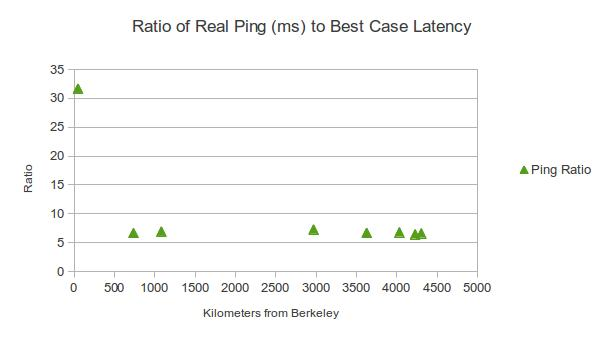
\includegraphics{RTT_chart}
\item[(b)] One reason that the Y values in this chart are greater than 2 is because even if there were the infrastructure set up to flawlessly deliver packets with no additional latencies and no queues or transmission delays, in order to meet the best case latency, there would have to be a direct line between any two points. Since every link must slightly deviate from the optimal line to reach its targets (taking a triangle or other shape to reach its destination), the latencies will be slower.

Another reason is the fact that there are other impediments to the delivery of packets than the speed of light; some examples are slower than the speed of light links, carrier policy slowing down packets, packet loss (and the subsequent re-sending of them), transmission delays, and queue delays (at particular endpoints). This is especially obvious with Stanford, which has the highest ratio. Because Stanford is very close to Berkeley, most of the delay does not actually come from the physical, speed of light transmission of the packet. Instead, there is a considerable amount of overhead in getting a packet out of Berkeley and on its way, and the subsequent routing amongst slow, probably heavily queued links in Palo Alto. This overhead is independent of the actual distance to the destination, and is less noticeable on packets sent to the East coast, where the propagation delay is actually the limiting factor (thanks to long distances).
\end{itemize}
\end{document}
